% ........................................................................... %

We now show how the prototype and protocol analysis approach can be used to facilitate service development on the following scenario. The scope of applications of protocol analysis goes however beyond just this example as we will see in the next chapter.
%
We assume here that a developer is defining a BPEL process, related to the handling of a purchase order, and that the process invokes several services during its execution. The tool will assist the developer in checking if the selected services have a protocol which is fully or partially compatible with the defined BPEL process, will identify which conversations can and cannot be carried out, and will also tackle the case of non compatibility by supporting the development of protocol adapters.

% ........................................................................... %

\section{BPEL process outline}

% ........................................................................... %

\begin{figure}[tbhp]
    \centering
    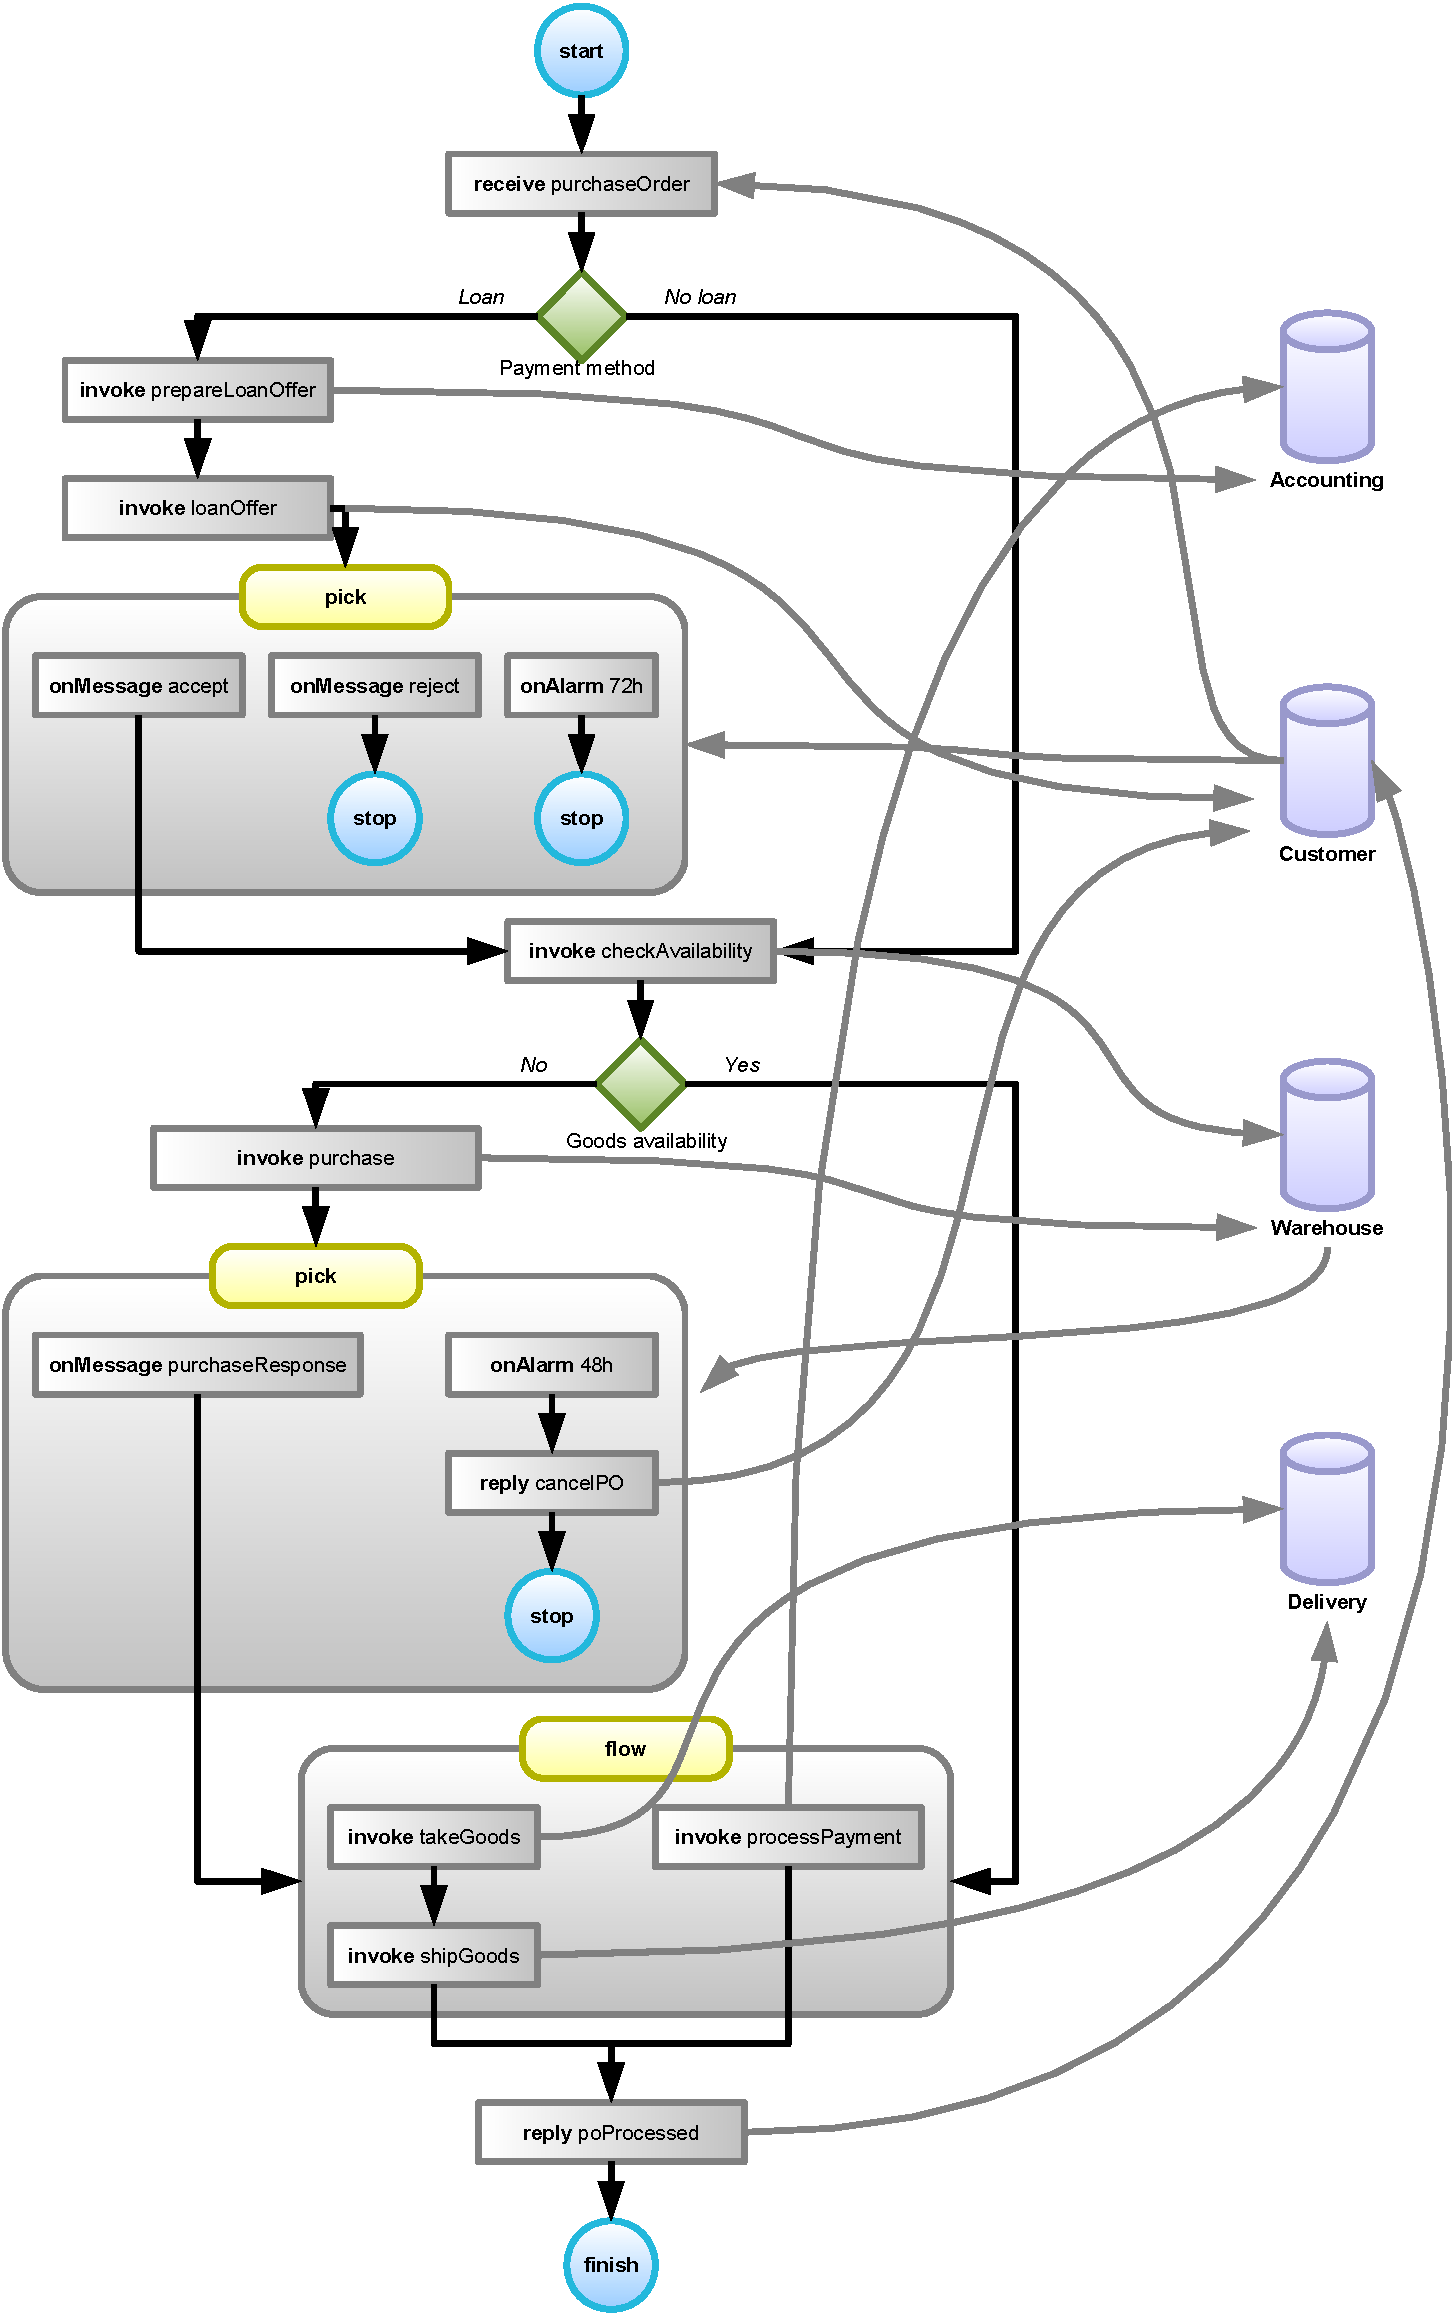
\includegraphics[height=\textheight]{content/sample-usecase/bpel-process}
    \caption{Simplified view of a BPEL process that handles purchase orders.}
    \label{fig:bpel-process}
\end{figure}

Consider the BPEL process depicted on Figure~\ref{fig:bpel-process}. It orchestrates four web services to process a purchase order. For the sake of clarity, we have removed the \emph{assign} BPEL instructions from the process diagram, normally required to prepare and reuse the messages exchanged with the involved web services. The first part of the process handles the payment options. If the customer asks for a loan, then the process will make an offer using the \emph{accounting} web service. The customer can then accept or reject it. The asynchronous \emph{pick} BPEL construction defines an alarm that will be fired after 72 hours to discard the process instance if the customer does not reply in time to the loan offer. The second part checks for the ordered goods availability with the warehouse web service. If some goods are not available, they will be ordered. In order to match quality of service requirements, the purchase is  canceled if the warehouse does not manage to purchase the missing goods within 48 hours. The third an last part of the process handles the payment and prepares the goods delivery. Finally, the customer is notified that the purchase has successfully completed.

% ........................................................................... %

\section{Business protocols extraction}

% ........................................................................... %

\begin{figure}[tbhp]
    \centering
    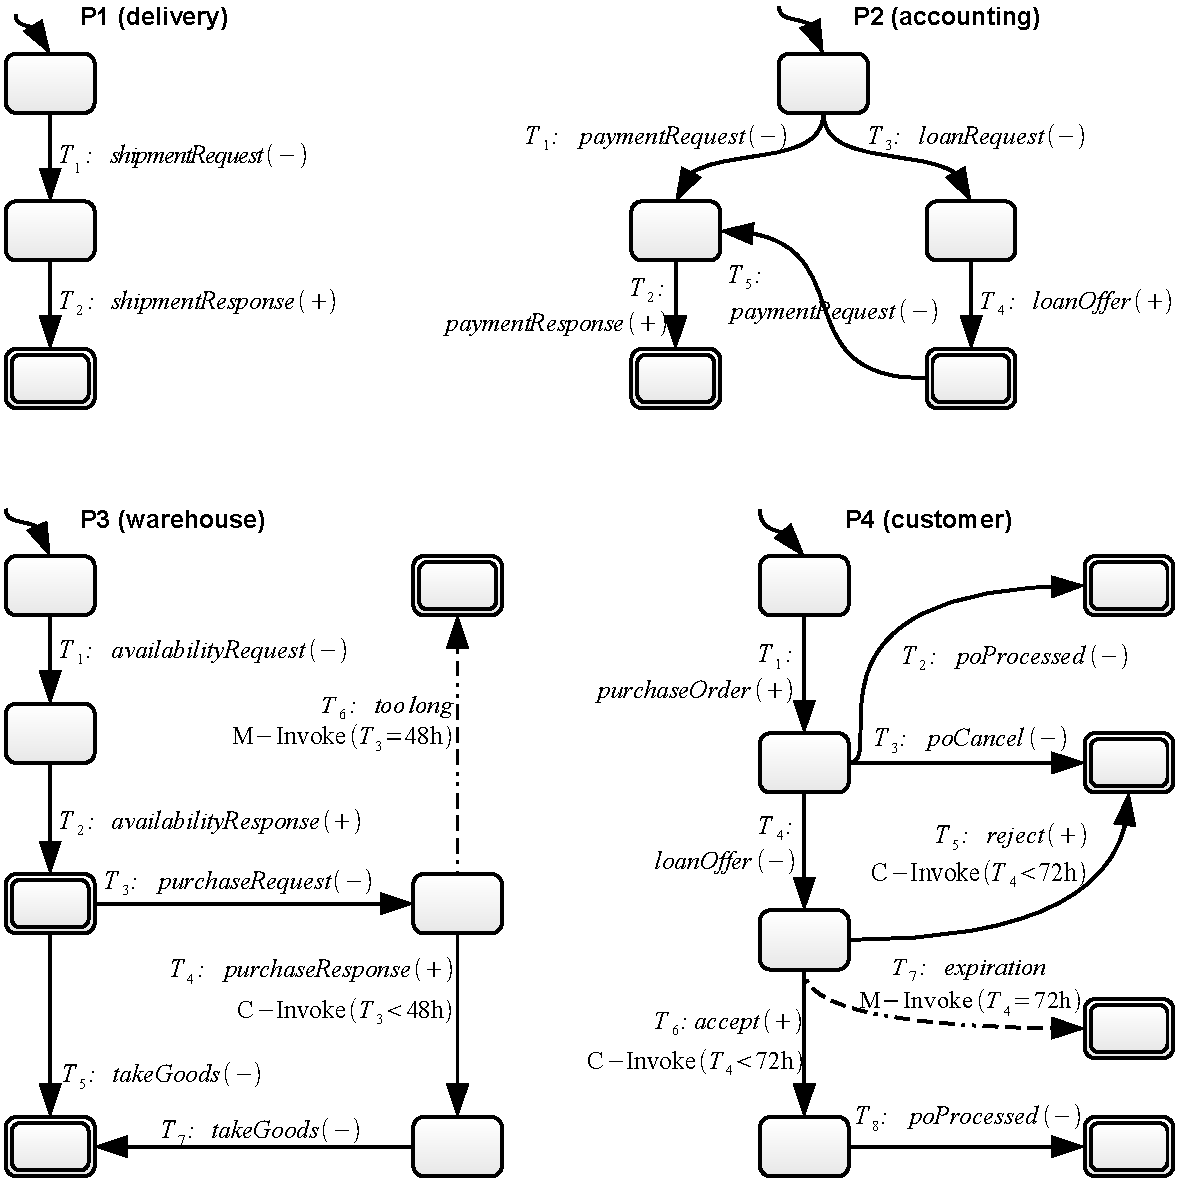
\includegraphics[width=\textwidth]{content/sample-usecase/bpel-protocols}
    \caption{Timed protocols extracted from the BPEL process of Figure~\ref{fig:bpel-process}.}
    \label{fig:bpel-protocols}
\end{figure}

Based on this BPEL process definition, we extract the timed protocols that the process supports when interacting with its partner services.
To do this, we use our multi-party protocol BPEL extractor, and we then obtain the protocol governing the interaction of the process with each of the partner services by filtering the multi-party protocol based on each service partner link.
The resulting protocols are shown in Figure~\ref{fig:bpel-protocols}.
Figure~\ref{fig:bpel-complete-warehouse} shows instead the protocol of the warehouse service we are planning to use as one of the services invoked by our process.

\begin{figure}[tbhp]
    \centering
    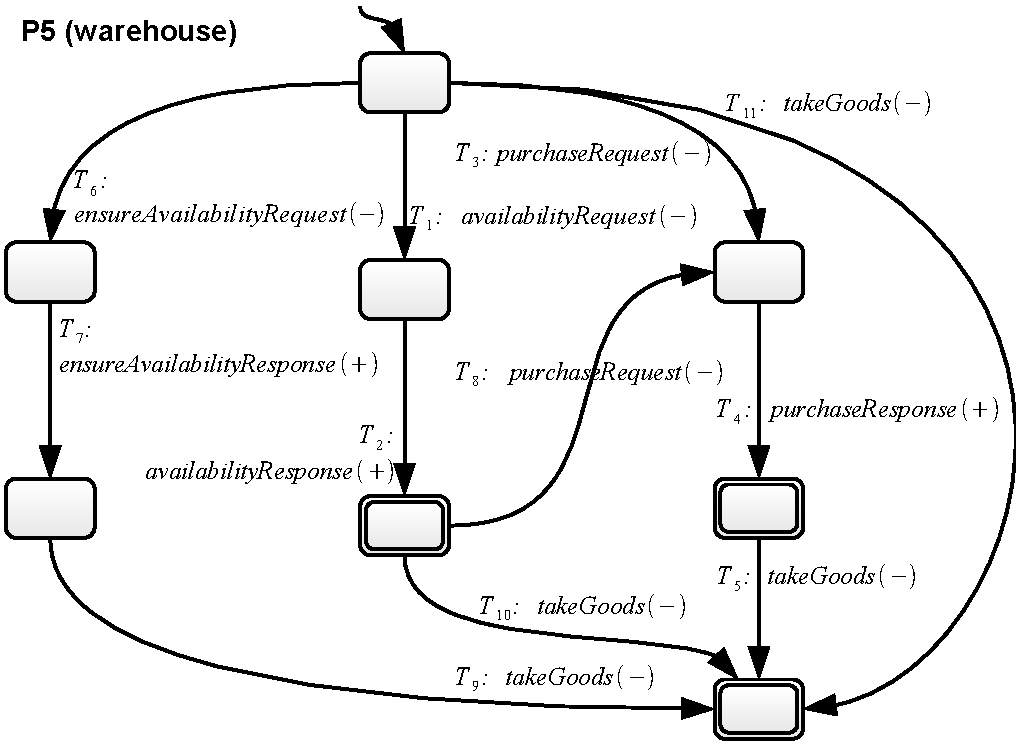
\includegraphics[width=\textwidth]{content/sample-usecase/bpel-warehouse-protocol}
    \caption{The complete warehouse service protocol.}
    \label{fig:bpel-complete-warehouse}
\end{figure}

% ........................................................................... %

\section{Protocol analysis}

% ........................................................................... %

\begin{figure}[tbhp]
    \centering
    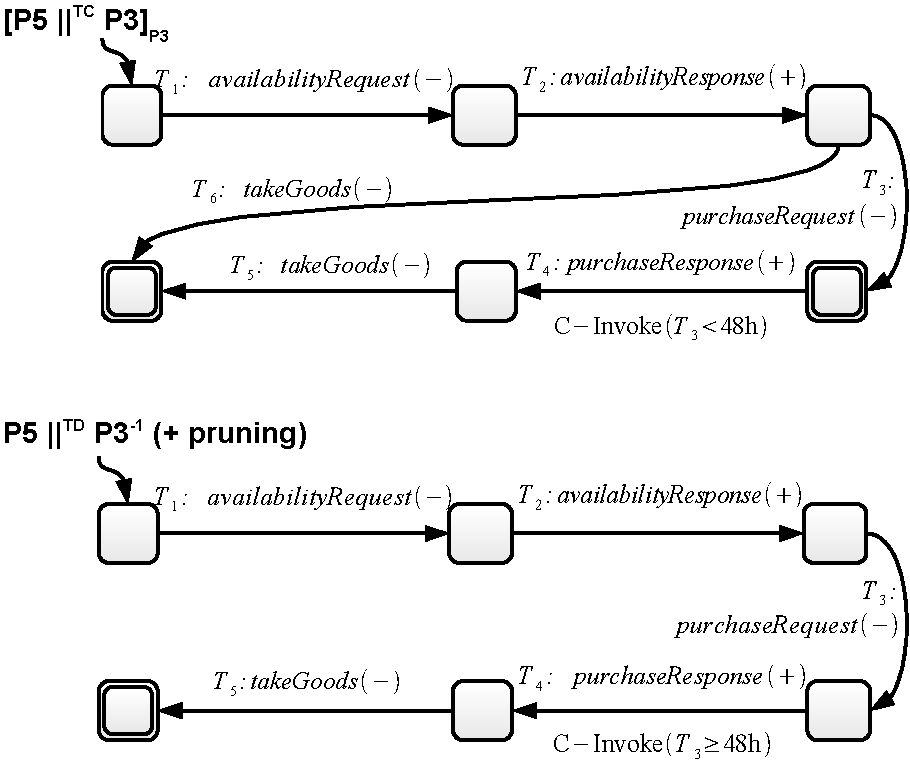
\includegraphics[width=\textwidth]{content/sample-usecase/bpel-warehouse-protocol-diff}
    \caption{Analysis of the common and differing conversations supported by $P_3$ and $P_5$.}
    \label{fig:bpel-warehouse-diff}
\end{figure}

We next apply the protocol analysis operators to assess compatibility between the protocols supported by our process and the protocols of the services we plan to use. For this, we assume that either the protocol or BPEL definition (from which we extract the protocol) of these services is available.
Figure~\ref{fig:bpel-warehouse-diff}) shows the results of this analysis for the warehouse service. In particular,
the compatible composition operator $P_5 \intersop P_3$ gives the set of the conversations that can occur between protocols $P_3$ and $P_5$.
Ideally, we would want this set to be equal to the conversations supported by $P_3$, which means that $P_5$ is fully compatible with $P_3$.\\

However, in our example, we do not have such luck. In fact we see that the conversations supported by the compatible composition are a subset of those supported by $P_3$.
The Figure further shows the conversations that are supported by the process but not by our partner service $P_5$ (which is empty in case of full compatibility), as well as the conversations that the partner supports but that the process does not support. The first of these two combined protocol is obtained by computing the inverse $P_3'$ of $P_3$ and then the difference $P_3^{-1} \diffop P_5$. The latter is instead computed as  $P_5 \diffop P_3^{-1}$. As we will examine later, all these combined protocols will become helpful in examining if and which changes need to be made to the process.\\

In particular, while the first combined protocol of  Figure~\ref{fig:bpel-warehouse-diff} (compatible composition) tells us what we can do, the second one denotes what our process is prevented from doing when using this partner (hence we call these \emph{prevented interactions}), while the third one denotes conversations that the partner would support, but we are not leveraging due to how we implemented the process. We call these \emph{neglected interactions}.\\

It is interesting to note that no compatibility problem would have been spotted in the case of business protocols without timing constraints \cite{FTBB}. Indeed, the untimed version of $P_5$ would have supported all of the conversations of the untimed version of $P_3$.

% ........................................................................... %

\section{Managing partial replaceability scenarios}

% ........................................................................... %

By looking at the three combined protocols, the developer can assess if the selected service is a good fit or not, and how to handle situations of partial replaceability or of no replaceability.
In general, this depends on the specific business purpose of the process. For example, the service I am planning to invoke may not support a $cancelPO$  operation, but I may be willing to take the risk and use it anyways even if cancellations are not allowed, for example because it offers cheaper rates.
Or, conversely, the selected service supports several forms of payments (accessed via different protocols) but my process can only support one of them, and we may be fine with it as for example our company only issues payments via credit card and not via bank transfers.\\

Alternatively, we can modify the process definition to adapt it to the service we are using, either to:
\begin{enumerate}
  
  \item ensure that our process does not generate conversations our partner cannot understand, or
  
  \item leverage conversations supported by our selected services (e.g., extend our process to support bank transfers).
  
\end{enumerate}

As another example, in our process, we can remove the \emph{onAlarm 48h} handler of the second \emph{pick} complex activity, so that the process will wait for the $purchaseResponse$ message to arrive, thereby removing the problematic temporal constraints in the extracted expected warehouse protocol. However, the process may find itself being put on hold indefinitely if a problem occurs on the warehouse service and it does not send a $purchaseResponse$ message back.\\

Another solution is to generate a protocol adapter \cite{BenatallahCGNT05} to reconcile the differences.
It can be done with the ServiceMosaic tools using an aspect-oriented framework \cite{KongdenfhaSBC06} where adapters are plugged through \emph{advices} written in BPEL. The adapter is be developed as follows. The \emph{pointcut} is triggered when a $purchaseRequest$ message is received. The advice is a BPEL process where an alarm starts counting from the reception of the $purchaseRequest$ message. If the service does not send a $purchaseResponse$ withing the next 48 hours, then the adapter drops it when the warehouse service sends it afterwards. The BPEL engine will have already woken up the process instance by then, and taken action by replying to the client partner link with a $cancelPO$ message.\\

Finally, it should be noted that for most BPEL engines, a message is simply dropped when it cannot be dispatched to any process instance for which it is waiting. An exception is then usually raised and logged inside the BPEL engine. In this example the adapter would be useful for diminishing the number of internally-thrown exceptions (raising exceptions has a significant performance cost). The choice of developing this adapter should be balanced in light of its development cost compared to the (limited) benefits, as BPEL engines can provide a form of ``implicit'' adapter in very specific mismatches cases such as this one.

% ........................................................................... %
